\documentclass[10pt]{examdesign}
\usepackage{amsmath}
\usepackage{pifont}
\usepackage{graphicx}
\SectionFont{\large\sffamily}
\Fullpages
\ContinuousNumbering
%\ShortKey
\setrandomseed{8282023}

\DefineAnswerWrapper{}{}
\NumberOfVersions{3}
\OneKey
\NoRearrange
\class{MAT 2000: Introduction to Statistics \\ Grace College}
\examname{Quiz 1.1-3}
\def\namedata{Name : \hrulefill}

\begin{document}
		
	\begin{multiplechoice}
		Do red uniform wearers tend to win more often than those wearing blue uniforms in tae-kwon-do matches where competitors are randomly assigned to wear either a red or blue uniform? In a sample of 80 tae-kwon-do matches, there were 45 matches where the red uniform wearer won.
		
		Refer to this scenario for questions 1-4
		\begin{question}
			\label{twd1} What is the parameter of interest for this study?
				\choice[!]{The long-run proportion of tae-kwon-do matches in which the red uniform wearer wins}
				\choice{45/80 of tae-kwon-do matches in which the red uniform wearer wins}
				\choice{Whether the red uniform wearer wins a match}
				\choice{0.50}
		\end{question}
		
		\begin{question}
			 \label{twd2} What is the statistic for this study?
				\choice{The long-run proportion of tae-kwon-do matches in which the red uniform wearer wins}
				\choice[!]{45/80 of tae-kwon-do matches in which the red uniform wearer wins}
				\choice{Whether the red uniform wearer wins a match}
				\choice{0.50}
		\end{question}
		
		\begin{question}			
			\label{twd3} Given below is the simulated distribution of the number of "red wins" that could happen by chance alone in a sample of 80 matches. Based on this simulation, is the observed result statistically significant?
			\begin{center}
				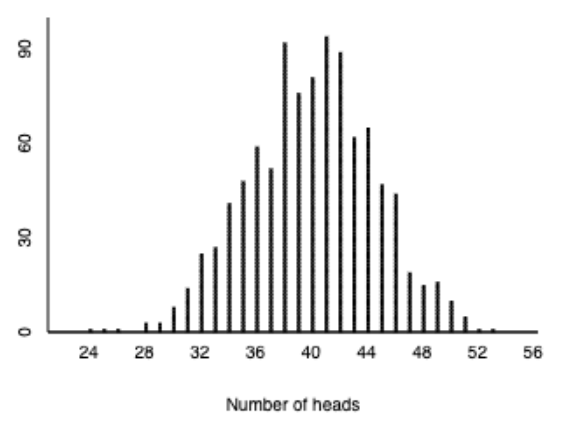
\includegraphics[width = 0.5 \linewidth]{sim1.png}
			\end{center}
				\choice{Yes, since 45 is larger than 40.}
				\choice{Yes, since the height of the dotplot above 45 is smaller than the height of the dotplot above 40.}
				\choice[!]{No, since 45 is a fairly typical outcome if the color of the winner's uniform was determined by chance alone.}
				\choice{No, since an observed value greater than 45 could just be by random chance.}
		\end{question}
		
		\begin{question}
			\label{twd4} What can be concluded from the results of this study? Select the option that does \textbf{NOT} apply.
				\choice{The results of this study are something that could easily have happened if the color of the winner's uniform was determined by chance alone.}
				\choice{Convincing evidence does not exist against the "by-chance-alone" model.}
				\choice[!]{The results of this study prove that the color of the winner's uniform was determined by chance alone.}
				\choice{Convincing evidence does not exist that red uniform wearers tend to win more often than those wearing blue uniforms.}
		\end{question}
			
		\begin{question}
			A test is being performed to see whether a dog, Hope, understands pointing towards an object. Two objects are placed about 2.5 meters away, then the tester point towards one of the objects. In 20 trials, Hope goes to the correct object 13 times (or 65%).
			Finish filling in the blanks with the correct One Proportion applet inputs to carry out an appropriate simulation of this process, if Hope does not understand pointing towards an object and is just guessing.
			\begin{itemize}
				\item Probability of success: \_\_\_(1)\_\_\_\_
				\item Sample size: \_\_\_(2)\_\_\_\_
				\item Number of samples: 10,000
			\end{itemize}
			\choice{0.65, 13}
			\choice{0.65, 20}
			\choice{0.5, 13}
			\choice[!]{0.5, 20}
		\end{question}
	
	\end{multiplechoice}
	
\end{document}
